%!TEX TS-program = XeLaTeX
%!TEX TS-program = XeLaTeX
\documentclass[11pt]{article}

\usepackage{amssymb}
\usepackage{amsthm}
\usepackage{amsmath}
\usepackage{mathtools}

\usepackage{fancyhdr}
\usepackage{graphicx}
\usepackage[top=3cm, left=2cm, right=2cm, headheight = 90pt]{geometry}
\usepackage{xltxtra}
\usepackage[font=small,labelfont=bf]{caption}

\usepackage{multicol}

\renewcommand{\theenumi}{\alph{enumi}}


\def\leq{\leqslant}
\def\geq{\geqslant}
\def\N{\mathbb N}
\def\R{\mathbb R}
\def\Z{\mathbb Z}
\DeclarePairedDelimiter\set\{\}

\def\prob{}

\theoremstyle{definition}
\newtheorem{problem}{\prob}


\pagestyle{fancy}

%!TEX TS-program = XeLaTeX

\fancyfoot[CE,CO]{}  % this is to remove page numbers (as you might want for single page docs)

%%!TEX TS-program = XeLaTeX
\renewcommand{\figurename}{Attēls}


\fancyhead[C]{{\Large\bf Coloring method - Solutions}\\ \date}

\begin{document}

\noindent 
%\emph{\notes}

%1
\begin{problem}
\textit{[Chess knight game]}

\textbf{Problem}

Alice and Bob plays a game:

First Alice places a chess knigth on any square on a chess-board. Then they take turns (starting with Bob) moving the knight according to chess rules, but they are not allowed to move to a square that has already been visited.

Which player has a winning strategy?

\textbf{Solution}

Divide the chessboard into $2 \times 4$ pieces like this
\begin{center}
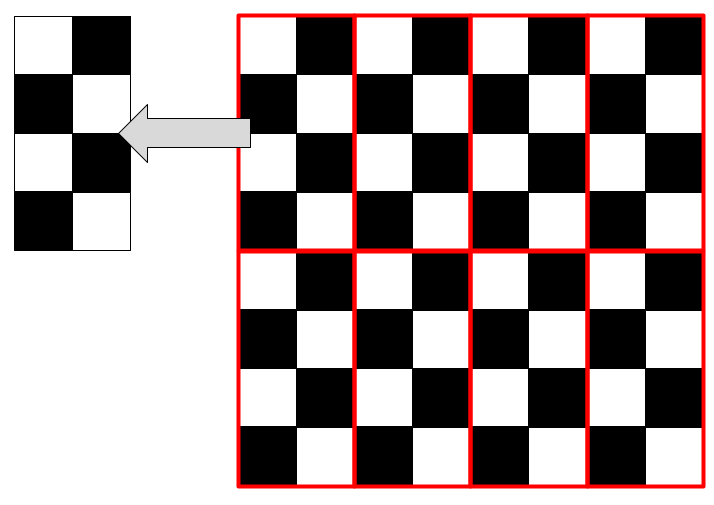
\includegraphics[width=6cm]{division.png}
\captionof{figure}{Division of chessboard }
\label{fig:divisionOfChessboard}
\end{center} 

\begin{center}
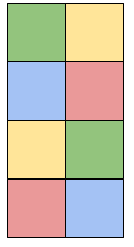
\includegraphics[width=1cm]{coloring.png}
\captionof{figure}{Coloring}
\label{fig:coloring}
\end{center} 

\end{problem}
%



\end{document}
